\chapter{Analiza wyników}
\thispagestyle{chapterBeginStyle}
\label{rozdzial5}

W ramach pracy dokonano szeregu testów przygotowanej implementacji algorytmu replikacji obrazów. Autor skupił się na tym, aby uzyskać jak najlepsze wyniki, stąd zdecydował się jedynie do metody tworzenia kolejnego pokolenia jedynie z najlepszych osobników z bieżącej iteracji, z jednoczesną możliwością zbadania pewnych parametrów, które pozwolą na stworzenie pewnego schematu działania algorytmów oraz analizę jakości ich działania. Jako osobniki \textit{najlepsze} należy rozumieć te, które są najbardziej \textit{podobne} do obrazu oryginalnego pod względem wartości funkcji celu (funkcja celu jest dla nich jak najmniejsza). Drugorzędnym kryterium oceny była w tym przypadku ocena wizualna. Obranie takiego kryterium wyboru osobników do utworzenia każdego kolejnego pokolenia wynika z faktu, że algorytm do oceny poszczególnych rozwiązań używa regularnej funkcji celu, która posiada lokalne optima z niewielką amplitudą.

W tym rozdziale zostaną przedstawione i omówione przeprowadzone testy. Autor skupił się tutaj na przedstawieniu postawionych hipotez odnośnie wpływu poszczególnych parametrów na jakość uzyskiwanych rozwiązań, analizie i prezentacji uzyskanych wyników oraz wyciągniętych na ich podstawie wniosków odnośnie zależności jakości uzyskiwanych obrazów a danym parametrem. 

Większość prezentowanych w tym rozdziale przykładów będzie opierać się na obrazie \textit{Mona Lisa} autorstwa Leonarda da Vinci, a dokładniej - na jego zdjęciu. Autor zdecydował się na wykorzystanie tego dzieła malarskiego ze względu na fakt, że jest to jeden z popularniejszych obrazów, które są wykorzystywane do prezentowania rezultatów w podobnych implementacjach dostępnych w sieci. Ma to na celu umożliwienie porównania czytelnikowi możliwości zaimplementowanego algorytmu z innymi dostępnymi rozwiązaniami wykorzystującymi podobne lub te same techniki.

\section{Rozmiar populacji}
\label{sec:population}
Dla problemu wpływu rozmiaru pojedynczej populacji na jakość otrzymywanych wyników autor pracy postawił następującą hipotezę:

\begin{hypothesis}
Liczba osobników w każdym pokoleniu wpływa na jakość ostatecznego rozwiązania zwracanego przez algorytm. Wraz ze wzrostem liczby osobników rośnie różnorodność osobników z unikalnym materiałem genetycznym, a przez co wzrasta również prawdopodobieństwo uzyskania osobników lepiej ocenianych przez funkcję celu.
\end{hypothesis}

W celu sprawdzenia powyższej hipotezy wykonano testy pozwalające zbadać wpływ parametru odpowiadającego za rozmiar pojedynczej populacji. Przeprowadzono testy na zdjęciu obrazu \textit{Mona Lisa} autorstwa Leonarda da Vinci zapisany jako plik \texttt{PNG} w skali RGBA - rysunek \ref{fig:mona_rgba}. Zbadano jak wpływa liczebność pojedynczego pokolenia dla określonej liczby iteracji na jakość uzyskanego rozwiązania.

\begin{figure}[!htb]
    \centering
    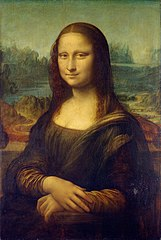
\includegraphics{images/mona/mona.jpg}
    \caption{
        Replikowany obraz \textit{Mona Lisa} w skali \texttt{RGBA}
        \textit{(Źródło: \cite{MonaLisa}})
    }
    \label{fig:mona_rgba}
\end{figure}

\subsection{Obserwacje}
Na rysunku \ref{fig:generations_1} przedstawiono jakość najlepszych rozwiązań (najlepiej ocenionych przez funkcję celu) po 1000 pokoleń odpowiednio dla 10, 50, 100 oraz 300 osobników w jednym pokoleniu. Zgodnie z tym, jak to opisano na początku niniejszego rozdziału, wybrano metodykę, w której każde kolejne pokolenie tworzone jest jedynie z \textit{pewnej} (określonej przez parametr podany przez użytkownika) liczby osobników, które zostały ocenione najwyżej przez funkcję celu. W tym, konkretnym przypadku dla takich osobników funkcja celu będzie miała wartość najmniejszą, co świadczy o fakcie, że odległość pomiędzy tymi rozwiązaniami a obrazem oryginalnym jest najmniejsza. Widoczna jest jedna znacząca różnica pomiędzy poszczególnymi prezentowanymi osobnikami pod względem wizualny. Na osobniku, który pochodził z testu, gdzie na pokolenie przypadało 300 osobników, można zauważyć wyraźny zarys postaci oraz elementów tła. Podobnie jest dla osobnika pochodzącego z testu, gdzie na pokolenie przypadało 100 osobników. W przypadku, gdy pokolenia miały liczność odpowiednio 50 i 10 osobników zauważenie konturów tła i postaci jest już praktycznie niemożliwe. Obraz z testu, w którym kolejne populacje liczyły po 10 obrazów, po 1000 iteracji obraz, pod względem wizualnym, w żaden sposób nie przypomina obrazu, do którego replikacji algorytm dąży. 

\begin{figure}[!htb]
    \centering
    \begin{subfigure}[b]{0.3\textwidth}
        \centering
         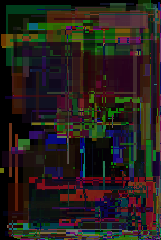
\includegraphics[width=\textwidth]{images/mona/10000_10_2/img_0_it_1000_best.png}
         \caption{10 osobników/pokolenie}
    \end{subfigure}
    \begin{subfigure}[b]{0.3\textwidth}
        \centering
         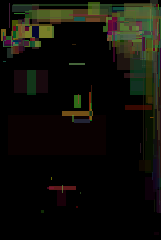
\includegraphics[width=\textwidth]{images/mona/10000_50_2/img_0_it_1000_best.png}
         \caption{50 osobników/pokolenie}
    \end{subfigure}
     \begin{subfigure}[b]{0.3\textwidth}
        \centering
         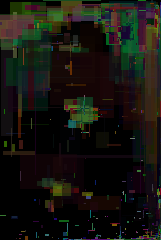
\includegraphics[width=\textwidth]{images/mona/10000_100_2/img_0_it_1000_best.png}
         \caption{100 osobników/pokolenie}
    \end{subfigure}
     \begin{subfigure}[b]{0.3\textwidth}
        \centering
         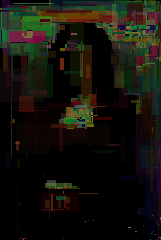
\includegraphics[width=\textwidth]{images/mona/10000_300_2/img_0_it_1000_best.png}
         \caption{300 osobników/pokolenie}
    \end{subfigure}
    \caption{Wyniki replikacji dla różnych liczności pokolenia dla 1000 iteracji algorytmu}
    \label{fig:generations_1}
\end{figure}


\subsection{Wnioski}
Zauważalna jest wyraźna wizualna różnica pomiędzy poszczególnymi zaprezentowanymi wynikami, dla różnych wartości parametru odpowiadającego za liczebność pokolenia, a obrazem zreplikowanym \ref{fig:mona_rgba}. Na podstawie prezentowanych wyników można stwierdzić, że liczebność pojedynczego pokolenia ma zdecydowany wpływ na jakość otrzymywanych rozwiązań - zarówno pod względem wizualnym, jak i względem wartości zwracanych przez funkcję celu. Potwierdza to postawione w hipotezie przypuszczenie, że wzrost liczby osobników powoduje, że różnorodność \textit{materiału genetycznego} jest większa (większa liczba osobników implikuje większą unikalność gwarantowaną przez operator mutacji). W takim przypadku algorytm wybiera osobniki do następnej iteracji z większej puli rozwiązań. Istnieje zatem większe prawdopodobieństwo zajścia mutacji (wzmocnionej potem przez operator krzyżowania) takiej, że osobnik z mutacją znacząco przybliży się, względem wartości funkcji oceny, do obrazu oryginalnego.

\section{Liczba pokoleń}
\begin{hypothesis}
Liczba pokoleń (iteracji) algorytmu wpływa na jakoś ostatecznego rozwiązania zwracanego przez algorytm. Wraz ze wzrostem liczby iteracji algorytmu zachodzi więcej zmian w materiale genetycznym osobników, przez co rośnie prawdopodobieństwo otrzymania rozwiązania bardziej zbliżonego, względem wartości funkcji celu, do obrazu replikowanego.
\end{hypothesis}

\subsection{Obserwacje}
W celu zbadania tego parametru ponownie zreplikowano obraz \ref{fig:mona_rgba}. Wyniki zaprezentowano na grafice \ref{fig:iterations_1}. Widoczna jest znacząca różnica pomiędzy rozwiązaniem uzyskanym po 100 iteracjach algorytmu, a rozwiązaniem uzyskanym w ostatniej, 10000., iteracji. Jednocześnie można zauważyć, że pomiędzy obrazem uzyskanym w 5000. iteracji, a osobnikiem z 10000. iteracji nie da się zauważyć, pod względem wizualnym, już wielu różnic.

\begin{figure}[!htb]
    \centering
    \begin{subfigure}[b]{0.3\textwidth}
        \centering
         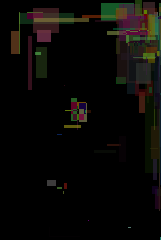
\includegraphics[width=\textwidth]{images/mona/10000_300_2/img_0_it_100_best.png}
         \caption{100 iteracji}
    \end{subfigure}
    \begin{subfigure}[b]{0.3\textwidth}
        \centering
         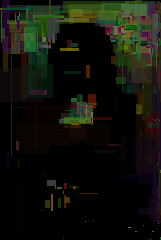
\includegraphics[width=\textwidth]{images/mona/10000_300_2/img_0_it_500_best.png}
         \caption{500 iteracji}
    \end{subfigure}
    \begin{subfigure}[b]{0.3\textwidth}
        \centering
         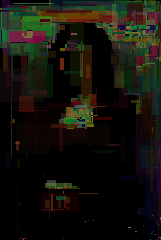
\includegraphics[width=\textwidth]{images/mona/10000_300_2/img_0_it_1000_best.png}
         \caption{1000 iteracji}
    \end{subfigure}
    \begin{subfigure}[b]{0.3\textwidth}
        \centering
         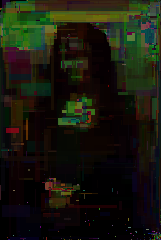
\includegraphics[width=\textwidth]{images/mona/10000_300_2/img_0_it_5000_best.png}
         \caption{5000 iteracji}
    \end{subfigure}
    \begin{subfigure}[b]{0.3\textwidth}
        \centering
         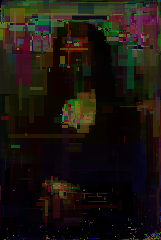
\includegraphics[width=\textwidth]{images/mona/10000_300_2/img_0_it_10000_best.png}
         \caption{10000 iteracji}
    \end{subfigure}
    \caption{Wyniki replikacji odpowiednio dla 100, 500, 1000, 5000 oraz 10000 iteracji algorytmu z liczebnością każdego pokolenia - 300 osobników}
    \label{fig:iterations_1}
\end{figure}

\subsection{Wnioski}
Na podstawie zaprezentowanych wyników można stwierdzić, że liczba iteracji algorytmu ma znaczący wpływ na jakość zwracanych rozwiązań. Wraz z każdą kolejną iteracją algorytmu widać, że z każdą kolejną iteracją zauważalna jest większa liczba podobieństw między konkretnym rozwiązaniem a obrazem replikowanym. Wynika to z faktu, że z każdą kolejną iteracją, genotyp poszczególnych osobników jest wzbogacany przez stosowane operatory genetyczne. Podobnie, jak ma to miejsce w przypadku opisanego w podrozdziale \ref{sec:population}, w tym przypadku również rośnie prawdopodobieństwo uzyskania obrazu bardziej zbliżonego do oryginału. Czynnikiem decydującym w tym przypadku jest nie ilość osobników w pojedynczym pokoleniu, ale liczba iteracji. Podobnie, jak ma to miejsce w naturalnym procesie ewolucji, z każdym kolejnym pokoleniem w osobnikach zachodzą zmiany genetyczne. Dysponując dużą pulą osobników można uzyskać wiele różnych zmian w genotypie, a powtarzając tę operację określoną liczbę razy, uzyskać wynik bardziej zbliżony do oryginalnego. Należy stwierdzić zatem, że zarówno parametr odpowiadający za liczbę pokoleń w algorytmie, jak i parametr odpowiedzialny za określenie mnogości każdego pokolenia, są ze sobą w ścisły sposób powiązane. 

Kolejnym wnioskiem, wynikającym z obserwacji dotyczącej niewielkich zmian pomiędzy 5000. a 10000. pokoleniem, jest to, że prezentowany algorytm replikacji może utknąć w lokalnym optimum. Oznacza to, że uzyskiwane odchylenia funkcji celu będą się mieścić w pewnym wąskim przedziale i nie będą się już znacząco powiększać. Od strony wizualnej, każde kolejne zmiany będą już praktycznie niezauważalne.

\section{Skala barw}
\begin{hypothesis}
Zastosowana w obrazie oryginalnym skala barw (rozważane są skala RGBA oraz skala szarości) ma pływ na jakość uzyskanych rozwiązań. Dla skali szarości (obrazy jednokanałowe) algorytm jest w stanie odtworzyć więcej szczegółów obrazu replikowanego, niż w przypadku zastosowania skali RGBA (obrazy czterokanałowe).
\end{hypothesis}
\begin{figure}[!htb]
    \centering
    \includegraphics[scale=4.0]{images/mona/mona_bw.jpg}
    \caption{Replikowany obraz \textit{Mona Lisa} w skali szarości (\textit{Źródło}: \cite{MonaLisa})}
    \label{fig:monra_bw}
\end{figure}
\subsection{Obserwacje}
W celu zaobserwowania różnic dla różnych skali barw dokonano replikacji obrazów \ref{fig:mona_rgba} oraz \ref{fig:monra_bw} dla takich samych parametrów wejściowych. Wyniki (dla 10000. pokolenia) zaprezentowano na grafice \ref{fig:scale_1}. Pod względem wizualnym, zauważalnym jest, że dla obrazu, który replikowany był w odcieniach szarości, widoczna jest większa liczba szczegółów, niż dla obrazu prezentowanego w skali RGBA. Porównywanie wartości funkcji celu, ze względu na dwie odmienne skale barw, zostanie tutaj pominięte.

\begin{figure}[!htb]
    \centering
    \begin{subfigure}[b]{0.3\textwidth}
        \centering
        \label{fig:scale_1_rgba}
         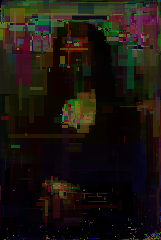
\includegraphics[width=\textwidth]{images/mona/10000_300_2/img_0_it_10000_best.png}
         \caption{Skala RGBA}
    \end{subfigure}
    \begin{subfigure}[b]{0.3\textwidth}
        \centering
        \label{fig:scale_1_bw}
         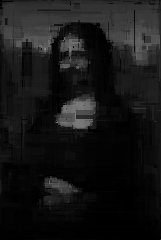
\includegraphics[width=\textwidth]{images/mona/10000_300_2/img_0_best.png}
         \caption{Skala szarości}
    \end{subfigure}
    \caption{Porównanie wyników replikacji dla skali szarości i RGBA \textit{ (10000 pokoleń, 300 osobników w pokoleniu}}
    \label{fig:scale_1}
\end{figure}

\subsection{Wnioski}
Wyniki replikacji w skali szarości pozwoliły na uzyskanie większej ilości szczegółów względem pierwowzoru, ze względu na fakt, że rozważany jest wówczas tylko jeden kanał i, w konsekwencji, podczas mutacji losowana jest tylko pojedyncza wartość. W przypadku skali RGBA takie wartości muszą być wylosowane cztery co jednocześnie zwiększa liczbę możliwych konfiguracji wartości dla wszystkich kanałów, przez co prawdopodobieństwa \textit{trafienia} w wartość koloru, który byłby jak najmniej oddalony od koloru danego piksela na obrazie oryginalnym maleje.

\section{Prawdopodobieństwo mutacji}
Kolejnym badanym parametrem, mającym wpływ na jakość uzyskanych rozwiązań był parametr odpowiadający za prawdopodobieństwo wystąpienia na danym osobniku mutacji. Ponownie zbadano wpływ parametru na jakość uzyskiwanych rozwiązań dla obrazu \ref{fig:mona_rgba}.

\begin{hypothesis}
Większa wartość parametru $p_{m}$ określającego prawdopodobieństwo wystąpienia mutacji wpływa na szybkość zbiegania algorytmu.
\end{hypothesis}

\subsection{Obserwacje}
Zbadano jakość uzyskiwanych rozwiązań dla parametru prawdopodobieństwa wystąpienia mutacji $p_{m} \in \lbrace 0.2, 0.4, 0.6, 0.8 \rbrace$. Wyniki przeprowadzonych testów zaprezentowano na grafice \ref{fig:mutation_1}. W tabeli \ref{tab:mutation_scores} przedstawiono wartości funkcji celu dla poszczególnych parametrów. Widoczne jest malenie wartości funkcji celu $f_{c}$ wraz ze wzrostem wartości parametru $p_{m}$. Pod względem wizualnym również daje się zauważyć, że na obrazach, gdzie prawdopodobieństwo wystąpienia mutacji było większe, odwzorowanie jest bardziej szczegółowe i na obrazach tych wyraźniej widoczna jest sylwetka postaci z obrazu będącego ich pierwowzorem.

\begin{table}[h]
    \centering
    \begin{tabular}{|c|c|}
        \hline
        $p_{m}$ & $f_{c}$  \\
        \hline
        $0.2$ & $496634177696466.0$ \\
        \hline
        $0.4$ & $496634145298532.0$ \\
        \hline
        $0.6$ & $496634099405528.0$ \\
        \hline
        $0.8$ & $496633985597704.0$ \\
        \hline
    \end{tabular}
    \caption{Wartości funkcji celu dla różnych wartości parametru $p_{m}$ określającego prawdopodobieństwo wystąpienia mutacji. Wyniki dla obrazów prezentuje rysunek \ref{fig:mutation_1}.}
    \label{tab:mutation_scores}
\end{table}

\begin{figure}[!htb]
    \centering
    \begin{subfigure}[b]{0.3\textwidth}
        \centering
        \label{fig:mutation_0_2}
         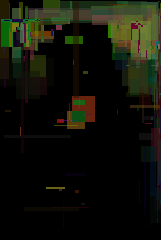
\includegraphics[width=\textwidth]{images/mona/1000_300_2/mutation/0_2.png}
         \caption{$p_{m} = 0.2$}
    \end{subfigure}
    \begin{subfigure}[b]{0.3\textwidth}
        \centering
        \label{fig:mutation_0_4}
         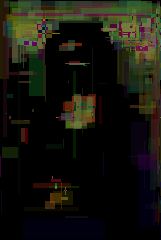
\includegraphics[width=\textwidth]{images/mona/1000_300_2/mutation/0_4.png}
         \caption{$p_{m} = 0.4$}
    \end{subfigure}
    \begin{subfigure}[b]{0.3\textwidth}
        \centering
        \label{fig:mutation_0_6}
         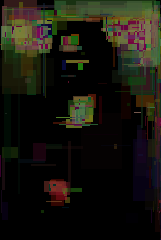
\includegraphics[width=\textwidth]{images/mona/1000_300_2/mutation/0_6.png}
         \caption{$p_{m} = 0.6$}
    \end{subfigure}
    \begin{subfigure}[b]{0.3\textwidth}
        \centering
        \label{fig:mutation_0_8}
         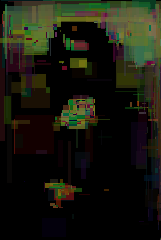
\includegraphics[width=\textwidth]{images/mona/1000_300_2/mutation/0_8.png}
         \caption{$p_{m} = 0.8$}
    \end{subfigure}
    \caption{Porównanie wyników replikacji dla różnych wartości parametru $p_{m}$ określającego prawdopodobieństwo mutacji \textit{1000 iteracji, 300 osobników w pokoleniu}}
    \label{fig:mutation_1}
\end{figure}

\subsection{Wnioski}
Na podstawie przedstawionych obserwacji łatwo zauważyć, że większa wartość parametru określającego prawdopodobieństwo wystąpienia mutacji w danym osobniku pozytywnie wpływa na jakość uzyskiwanych rozwiązań. Im większe prawdopodobieństwo mutacji, tym większa szansa, że do genotypu danego osobnika zostanie wprowadzona \textit{pozytywna} zmiana. Przez \textit{pozytywną} zmianę rozumie się taką, która sprawie, że odległość pomiędzy wygenerowanym rozwiązaniem, a obrazem oryginalnym zmniejsza się w stosunku do stanu, zanim mutacja została wprowadzona. Należy też w tym miejscu zauważyć, że większa wartość parametru $p_{m}$ niekoniecznie musi gwarantować uzyskanie lepszych wyników. Może bowiem dojść do takiej sytuacji, że genotyp osobników będzie w taki sposób modyfikowany, że zmiany nie będą korzystne dla oczekiwanych rezultatów, to jest mogą zostać wprowadzone zmiany, które sprawią, że osobniki w kolejnym pokoleniu mogą zostać ocenione gorzej od osobników z pokolenia poprzedniego.

\section{Liczba osobników wybieranych do utworzenia populacji}
W następnej kolejności zbadano wpływ liczby osobników wybieranych jako najlepsze w danym pokoleniu do utworzenia kolejnej populacji na jakość uzyskiwanych rozwiązań. 

\begin{hypothesis}
Wzrost liczby najlepiej przez funkcję celu ocenianych osobników wybieranych do następnego pokolenia zmniejsza prawdopodobieństwo zbiegania algorytmu do optymalnego rozwiązania.
\end{hypothesis}

\subsection{Obserwacje}
W tym przypadku autor ponownie zbadał to zjawisko na podstawie replikacji obrazu \ref{fig:mona_rgba}. Wyniki zaprezentowano na grafice \ref{fig:num_of_best}. Bardzo wyraźnie widać, że wraz ze wzrostem liczby osobników wybieranych do tworzenia kolejnego pokolenia zarys sylwetki widocznej na obrazie kobiety zaczyna być co raz mniej dostrzegalny. Dla 200 wybieranych osobników, po 1000 iteracji algorytmu na obrazie widać jedynie losowy szum, który zupełnie nie przypomina pierwowzoru. 

\begin{figure}[!htb]
    \centering
    \begin{subfigure}[b]{0.3\textwidth}
        \centering
        \label{fig:num_of_best_2}
         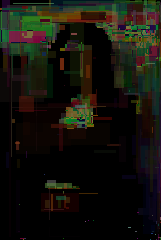
\includegraphics[width=\textwidth]{images/mona/num_of_best/2.png}
         \caption{2 osobniki}
    \end{subfigure}
    \begin{subfigure}[b]{0.3\textwidth}
        \centering
        \label{fig:num_of_best_10}
         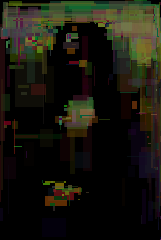
\includegraphics[width=\textwidth]{images/mona/num_of_best/10.png}
         \caption{10 osobników}
    \end{subfigure}
    \begin{subfigure}[b]{0.3\textwidth}
        \centering
        \label{fig:num_of_best_50}
         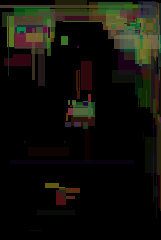
\includegraphics[width=\textwidth]{images/mona/num_of_best/50.png}
         \caption{50 osobników}
    \end{subfigure}
    \begin{subfigure}[b]{0.3\textwidth}
        \centering
        \label{fig:num_of_best_100}
         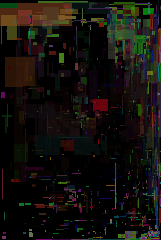
\includegraphics[width=\textwidth]{images/mona/num_of_best/100.png}
         \caption{100 osobników}
    \end{subfigure}
    \begin{subfigure}[b]{0.3\textwidth}
        \centering
        \label{fig:num_of_best_200}
         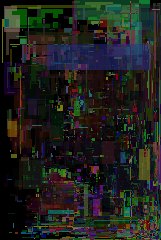
\includegraphics[width=\textwidth]{images/mona/num_of_best/200.png}
         \caption{200 osobników}
    \end{subfigure}
    \caption{Porównanie wyników replikacji dla różnej liczby osobników wykorzystanych do tworzenia nowego pokolenia \textit{(1000 pokoleń, 300 osobników w pokoleniu)}}
    \label{fig:num_of_best}
\end{figure}

\subsection{Wnioski}
Wraz ze wzrostem liczby osobników, z których jest tworzone kolejne pokolenie maleje czytelność uzyskiwanych wyników. Dla wartości parametru 2, 50 i 100 daje się jeszcze na obrazie rozróżnić sylwetkę kobiety z oryginalnego obrazu. W przypadku wartości 100 i 200 na obrazach widoczny jest jedynie losowy szum. Wynika to z faktu, że wraz ze wzrostem liczby wyselekcjonowanych osobników, do następnego pokolenia dostają się również osobniki gorzej ocenione przez funkcję celu. W konsekwencji tego wybór staje się bardziej losowy. Na podstawie obserwacji można stwierdzić, że im mniej osobników zostało wybranych do utworzenia nowej populacji, tym algorytm szybciej zbiega do oczekiwanego rozwiązania.

\section{Złożoność obrazu}
Ostatnim zbadanym czynnikiem, mogącym mieć wpływ na jakość uzyskiwanych wyników, a przez to - na szybkość zbiegania algorytmu, była złożoność replikowanego obrazu. 

\begin{hypothesis}
Wraz ze wzrostem liczby szczegółów na replikowanym obrazie maleje dokładność jego odwzorowania.
\end{hypothesis}

Postawioną powyżej hipotezę sprawdzono na kilku obrazach o różnym stopniu skomplikowania zaprezentowanych na grafice przedstawionych na rysunku \ref{fig:complexity_original}. Obraz \textbf{(a)} przedstawia zdjęcie twarzy wygenerowanej przez sztuczną inteligencję. Mimo sporej liczby szczegółów, twarz osoby obecnej na zdjęciu zajmuje sporą część zdjęcia przez to jest elementem zajmującym większość przestrzeni na obrazie. Ponadto obraz ten posiada jednokolorowe tło. Na \textbf{(b)} przedstawiona portret postaci w taki sposób, że jest ona widoczna do końca jej tułowia. Obraz zawiera sporo szczegółów w tle jak i na ubraniu, które ma na sobie sportretowana kobieta (zagięcia, cienie). Ostatni obraz \textbf{(c)}, zawiera wiele elementów o różnym stopniu jasności i skomplikowania.

\begin{figure}[!htb]
    \centering
    \begin{subfigure}[b]{0.3\textwidth}
        \centering
        \label{fig:complexity_ai}
         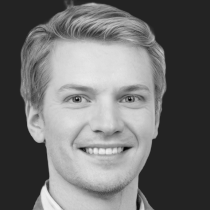
\includegraphics[width=\textwidth]{images/complexity/originals/ai2.png}
         \caption{Zdjęcie twarzy wygenerowane przez AI (\textit{Źródło}: \cite{AIFace})}
    \end{subfigure}
    \begin{subfigure}[b]{0.3\textwidth}
        \centering
        \label{fig:complexity_mona}
         \includegraphics[width=\textwidth]{images/complexity/originals/mona_bw.jpg}
         \caption{\textit{Mona Lisa}, Leonardo da Vinci (\textit{Źródło}: \cite{MonaLisa})}
    \end{subfigure}
    \begin{subfigure}[b]{0.8\textwidth}
        \centering
        \label{fig:complexity_guernica}
         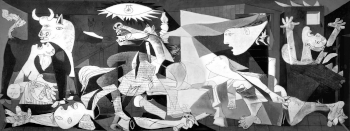
\includegraphics[width=\textwidth]{images/complexity/originals/gueranica_bw.png}
         \caption{\textit{Guernica}, Pablo Picasso (\textit{Źródło}: \cite{Guernica})}
    \end{subfigure}
    \caption{Obrazy o różnej złożoności pod względem liczby obecnych na nich szczegółów}
    \label{fig:complexity_original}
\end{figure}

\subsection{Obserwacje}
Wyniki replikacji obrazów przedstawia grafika \ref{fig:complexity_rep}. Widać, że algorytm poradził sobie najlepiej z obrazem \textbf{(a)}, na którym widoczna była sama twarz, a najgorzej z tymi, które wymagały odwzorowania wielu elementów o różnych rozmiarach. W przypadku dwóch pozostałych obrazów widać jedynie zarysy postaci. O ile w przypadku zreplikowanego obrazu \textbf{(b)} obserwator jest w stanie domyślać się, że jest to portret kobiety, o tyle w przypadku \textbf{(c)} ciężko stwierdzić co dokładnie zostało na obrazie przedstawione.

\begin{figure}[!htb]
    \centering
    \begin{subfigure}[b]{0.3\textwidth}
        \centering
        \label{fig:complexity_ai_rep}
         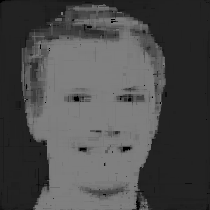
\includegraphics[width=\textwidth]{images/complexity/ai.png}
         \caption{Zdjęcie twarzy wygenerowane przez AI}
    \end{subfigure}
    \begin{subfigure}[b]{0.3\textwidth}
        \centering
        \label{fig:complexity_mona_rep}
         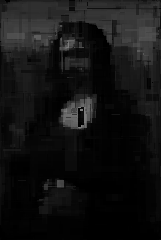
\includegraphics[width=\textwidth]{images/complexity/mona.png}
         \caption{\textit{Mona Lisa}, Leonardo da Vinci}
    \end{subfigure}
    \begin{subfigure}[b]{0.8\textwidth}
        \centering
        \label{fig:complexity_guernica_rep}
         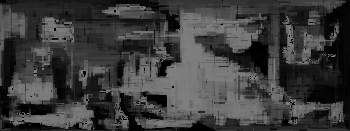
\includegraphics[width=\textwidth]{images/complexity/guernica.png}
         \caption{\textit{Guernica}, Pablo Picasso}
    \end{subfigure}
    \caption{Wyniki replikacji obrazów przedstawionych na \ref{fig:complexity_original} \textit{(10000 pokoleń, 300 osobników w pokoleniu)}}
    \label{fig:complexity_rep}
\end{figure}

\subsection{Wnioski}
Na podstawie przedstawionych obserwacji można wyciągnąć wnioski, że liczba szczegółów ma znaczący wpływ na szczegółowość odwzorowania obrazu. Przy okazji badania wpływu szczegółowości obrazu na jakość rozwiązania, warto zauważyć, że jest to również poniekąd związane z rozdzielczością obrazu. Im większy obraz, tym więcej szczegółów jest na nim widocznych.

\section{Czas działania programu}
Autor zbadał również zależność czasu działania algorytmu od dwóch najbardziej istotnych parametrów jakimi są liczba iteracji oraz rozmiar pojedynczego pokolenia. Wyniki zaprezentowano w tabelach \ref{tab:times_it} oraz \ref{tab:times_gen} (Testy przeprowadzono na systemie \texttt{macOS 10.15 Catalina} i sześciordzeniowym procesorze (16 wątków) Intel Core i7. Czas działania programu został zmierzony za pomocą konsolowego programu \texttt{time} dostępnego w systemach typu Unix-like).

\begin{table}[!htb]
    \centering
    \begin{tabular}{|c|c|c|}
        \hline
        $i$ & $N$ & $\mathrm{time}$ [$s$]  \\
        \hline
        $10000$ & $50$ & $294.52$ \\
        \hline
        $10000$ & $100$ & $540.48$ \\
        \hline
        $10000$ & $200$ & $1128.97$ \\
        \hline
        $10000$ & $300$ & $1731.64$ \\
        \hline
    \end{tabular}
    \caption{Czasy działania algorytmu (w sekundach) dla stałej liczby iteracji iteracji ($i$) oraz zmiennego rozmiaru pokolenia ($N$).}
    \label{tab:times_it}
\end{table}

\begin{table}[!htb]
    \centering
    \begin{tabular}{|c|c|c|}
        \hline
        $i$ & $N$ & $\mathrm{time}$ [$s$]  \\
        \hline
        $500$ & $200$ & $52.86$ \\
        \hline
        $1000$ & $200$ & $111.07$ \\
        \hline
        $5000$ & $200$ & $588.98$ \\
        \hline
        $10000$ & $200$ & $1731.64$ \\
        \hline
    \end{tabular}
    \caption{Czasy działania algorytmu (w sekundach) dla zmiennej liczby iteracji iteracji ($i$) oraz stałego rozmiaru pokolenia ($N$).}
    \label{tab:times_gen}
\end{table}

\subsection{Obserwacje}
Na podstawie przeprowadzonych obserwacji można zauważyć, że zarówno, gdy zmienia się rozmiar pokolenia przy stałej liczbie iteracji (tabela \ref{tab:times_it}), jak i w sytuacji, gdy zmianie ulega liczba iteracji, liczność pokolenia jest stała (tabela \ref{tab:times_gen}), czas działania programu rośnie wprost proporcjonalnie do zmieniającego się parametru.

\subsection{Wnioski}
W obu przypadkach wzrost czasu działania programy wynika z innej przyczyny. W sytuacji, gdy zmienia się jedynie rozmiar pokolenia, program wykonuje się dłużej, ponieważ w każdej iteracji potrzebuje więcej czasu na przetworzenie wszystkich osobników (zastosowanie operatorów mutacji i ocena). W przypadku, gdy stały jest rozmiar pokolenia, a zmienia się liczba iteracji fakt, że program działa dłużej wynika z tego, że chociaż w każdej iteracji przetworzenie wszystkich osobników w populacji zajmuje tyle samo czasu, ale wzrost jest spowodowany większą liczbą powtórzeń w programie.

\section{Parametry a ograniczenie czasowe}

Ostatnim elementem analizy jest zbadanie zależności pomiędzy liczbą iteracji i licznością pojedynczego pokolenia, w przypadku, gdy na algorytm zostało narzucone ograniczenie czasowe. Celem tego testu jest sprawdzenie, który parametr opłaca się zwiększyć (kosztem zmniejszenia wartości drugiego), aby uzyskać jak najlepsze wyniki. Autor przeprowadził testy na obrazie \ref{fig:monra_bw} dla różnych wartości liczby pokoleń algorytmu i rozmiaru populacji przy założeniu, że jest to zależność odwrotnie proporcjonalna (czas działania dla każdego był, w przybliżeniu, taki sam). Wyniki prezentuje grafika \ref{fig:dependence_rep}. Zbadane konfiguracje parametrów i czas działania programu dla każdej z nich przedstawiono w tabeli \ref{tab:dependence_times}. 

\begin{table}[!htb]
    \centering
    \begin{tabular}{|c|c|c|}
        \hline
        $i$ & $N$ & $\mathrm{time}$ [$s$]  \\
        \hline
        $10000$ & $50$ & $294.52$ \\
        \hline
        $5000$ & $100$ & $282.98$ \\
        \hline
        $1000$ & $500$ & $275.97$ \\
        \hline
        $500$ & $1000$ & $284.22$ \\
        \hline
    \end{tabular}
    \caption{Czasy działania algorytmu (w sekundach) dla różnych wartości liczby iteracji ($i$) oraz rozmiaru pojedynczego pokolenia ($N$). Testy przeprowadzono na systemie \texttt{macOS 10.15 Catalina} i sześciordzeniowym procesorze (16 wątków) Intel Core i7. Czas działania programu został zmierzony za pomocą konsolowego programu \texttt{time} dostępnego w systemach typu Unix-like.}
    \label{tab:dependence_times}
\end{table}

\begin{figure}[!htb]
    \centering
    \begin{subfigure}[b]{0.3\textwidth}
        \centering
        \label{fig:dependence_10000_50}
         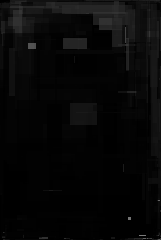
\includegraphics[width=\textwidth]{images/mona/dependence/10000_50.png}
         \caption{10000 pokoleń, 50 osobników w pokoleniu}
    \end{subfigure}
    \begin{subfigure}[b]{0.3\textwidth}
        \centering
        \label{fig:dependence_5000_100}
         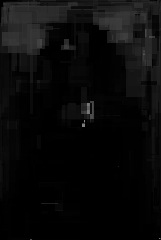
\includegraphics[width=\textwidth]{images/mona/dependence/5000_100.png}
         \caption{5000 pokoleń, 100 osobników w pokoleniu}
    \end{subfigure}
    \begin{subfigure}[b]{0.3\textwidth}
        \centering
        \label{fig:dependence_1000_500}
         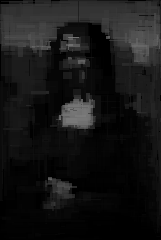
\includegraphics[width=\textwidth]{images/mona/dependence/1000_500.png}
         \caption{1000 pokoleń, 500 osobników w pokoleniu}
    \end{subfigure}
    \begin{subfigure}[b]{0.3\textwidth}
        \centering
        \label{fig:dependence_500_1000}
         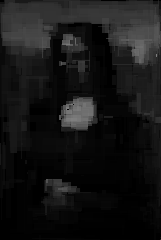
\includegraphics[width=\textwidth]{images/mona/dependence/500_1000.png}
         \caption{500 pokoleń, 1000 osobników w pokoleniu}
    \end{subfigure}
    \caption{Wyniki prezentujące zależność pomiędzy liczbą pokoleń algorytmu a licznością pokolenia}
    \label{fig:dependence_rep}
\end{figure}

\subsection{Obserwacje}
Można zauważyć, że czas działania dla każdej z konfiguracji parametrów jest w przybliżeniu taki sam (ponad 4 minuty). Na grafice \ref{fig:dependence_rep} widać wyraźnie, że wraz ze wzrostem liczby pokoleń i jednoczesnym zmniejszeniem liczby osobników w pokoleniu znacznie pogorszyła się, pod względem wizualnym, jakość uzyskanego rozwiązania. Uzyskany rezultat jest bardzo odległy od oczekiwanego - sylwetka postaci przedstawionej na obrazie oryginalnym jest prawie całkowicie niewidoczna.  Najlepsze wyniki uzyskano dla przypadku, gdy ograniczono liczbę iteracji algorytmu (do 1000-500) a zwiększono liczbę osobników tworzących dane pokolenie - na tych obrazach wyraźnie można wyróżnić prezentowaną na obrazie postać oraz zarysy elementów tła.

\subsection{Wnioski}
Na podstawie przeprowadzonych obserwacji można stwierdzić, że w przypadku, gdy wymagane jest narzucenie ograniczenia czasowego na program, lepszym wyborem będzie zwiększenie liczby osobników w pokoleniu kosztem zmniejszenia liczby iteracji programu. 

\section{Podsumowanie}
W niniejszym rozdziale dotyczącym analizy uzyskanych wyników przedstawiono wyniki testów, które miały zbadać wpływ możliwych do ustawiania przez użytkownika parametrów, które, potencjalnie, mogą mieć największy wpływ na jakość uzyskiwanych rozwiązań. Po analizie przedstawionych obserwacji oraz wniosków można zauważyć, że algorytm lepiej radzi sobie z obrazami, zawierającymi mniej szczegółów oraz w jednolitej skali kolorystycznej - skali szarości. Obserwator może również stwierdzić, że algorytmowi trudniej odwzorować obszary ciemniejsze, a dokładniejsze odwzorowanie pierwowzoru otrzymuje się w przypadku obrazów jaśniejszych. W kontekście możliwych rozszerzeń pracy należałoby przebadać jakość uzyskiwanych rozwiązań dla, na przykład zdjęć zrobionych w dobrych warunkach oświetleniowych, obrazów namalowanych w jasnych kolorach lub zdjęć prześwietlonych.

Autor chce zauważyć, że jest to jedynie niewielka część różnych zestawień konfiguracji algorytmu, które mogłyby zostać zbadane. Zdecydował się on na zaprezentowanie jedynie tych, które według jego uznania pokazywały w najlepszy sposób zarówno mocne, jak i słabe strony opisywanego algorytmu. Ze względu małej ilości czasu autorowi nie udało się przeprowadzić wszystkich zamierzonych testów. Sugerowane ścieżki testowania i oceny generowanych rozwiązań to:
\begin{itemize}
    \item zbadanie subiektywnej oceny osób trzecich w postaci ankiety i późniejsza jej analiza,
    \item zbadanie innych metryk oceny jakości rozwiązań (funkcja celu),
    \item zbadanie jak algorytm poradzi sobie z obrazami w dużych rozdzielczościach, na przykład \textit{FullHD},
    \item zbadanie dokładnego profilowania pamięci podczas działania programu, na przykład za pomocą narzędzia \texttt{Valgrind}.
\end{itemize}
